\chapter{Matlab Tool}

The presented tool uses the Symbolic Math Toolbox\footnote{http://www.mathworks.ch/products/symbolic/}. 

\section{Kinematic Tree}\label{sec:kintree}
The robot is described as a kinematic tree.  
A root element needs to be selected first and from there the individual branches are successively described.
Each rigid body has to be described with the following struct:


\begin{lstlisting}
% => start setting up the kinematic structure.  Each link needs to have all the folowing struct elements 
% B indicates bodyframe
% P indicates coordinate system of parent element

% body(i).param.m: 			 body mass
% body(i).param.B_Th: 	 inertia tensor in body frame w.r.t. CoG
% body(i).param.B_r_COG: CoG in body frame
% body(i).cs.P_r_PO:		 position of origin in parent CS
% body(i).cs.A_PB:  		 rotation from parent CS
% body(i).tree.parent:   tree parent (0=inertial frame)

%% Body 1
i = 1;
% body mass
body(i).param.m = m1;   
body(i).param.B_Th = diag([Th1_xx Th1_yy Th1_zz]); 
body(i).param.B_r_COG = [0;0;s1];
body(i).cs.P_r_PO = sym([0;0;0]); % ensure a symbolic expression
body(i).cs.A_PB = eulerToRotMat_A_IB(0,0,q1);
body(i).tree.parent = 0;
\end{lstlisting}
Some notes on the notation:\\
\begin{tabular}{ll}
$_B\boldsymbol{\theta}$: & Inertia of the body with respect to CoG expressed in body fixed frame B\\
$_B\mathbf{r}_{CoG}$: & Vector from origin of body fixed frame to CoG expressed in body frame B\\
$_P\mathbf{r}_{PO}$: & Translational vector from origin of parent frame P \\ & to origin of body frame B expressed in parent frame P \\
$\mathbf{A}_{PB}$: & Rotation matrix that rotates a vector expressed in body frame B to parent frame P
\end{tabular}
See Figure~\ref{fig:3D_PR}, which represents a 3-link robot arm, to better understand the definition of the vectors.
\clearpage
\section{Force Elements}\label{sec:forceel}
This framework allows to describe both force (prismatic, type = 'lin') and torque (rotational, type='rot') actuators.  

\begin{figure}[H]
	\centering
		\subfigure[Torque actuator acting in a revolute joint (type = 'rot').]{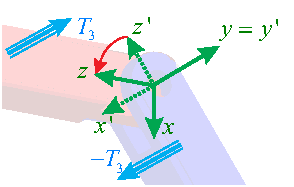
\includegraphics[width=0.3\textwidth]{../RobotArmExample/revoluteJoint.pdf}}\qquad\qquad
		\subfigure[Force actuator acting in a prismatic joint (type = 'lin').]{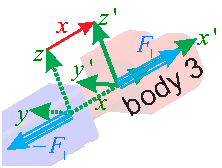
\includegraphics[width=0.3\textwidth]{../RobotArmExample/linearJoint.pdf}}
		%\subfigure[Torque actuator acting in a revolute joint (type = 'rot').]{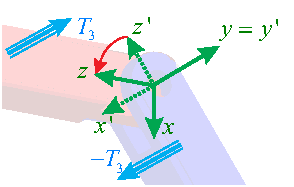
\includegraphics[width=0.3\textwidth]{../RobotArmExample/revoluteJoint.pdf}}\qquad\qquad
		%\subfigure[Force actuator acting in a prismatic joint (type = 'lin').]{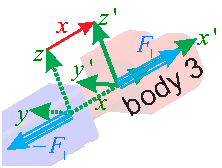
\includegraphics[width=0.3\textwidth]{../RobotArmExample/linearJoint.pdf}}
	\caption{Two types of force elements can be defined.}
	\label{fig:joints}
\end{figure}

\subsection{Torque Actuators} \label{sec:torqueAct}

This is the most common actuator for all types of robotic arms.  They are defined as follows:
\begin{lstlisting}
% torque element acting between environment and body 1
i = 1;
ftel(i).type = 'rot';       % define it to be a rotational = torque 
ftel(i).body_P = 0;         % body on which the reaction happens
ftel(i).body_B = 1;         % body on which the action happens
ftel(i).B_T = [0;0;T1];     % torque vector, expressed in B frame
\end{lstlisting}
For a detailed example, please check \secref{sec:3link}.

\subsection{Force Actuators}
Prismatic joints (like hydraulic/pneumatic cylinders, spindle drives, etc.) are defined as follows:
\begin{lstlisting}
% force element acting between body 2 and body 3
i = 3;
ftel(i).type = 'lin';        % define it to be a rotational = torque 
ftel(i).body_P = 2;          % body on which the reaction happens
ftel(i).body_B = 3;          % body on which the action happens
ftel(i).P_r_R = sym([0;0;0]);% point of reaction in P frame
ftel(i).B_r_A = sym([0;0;0]);% point of action in B frame
ftel(i).B_F = [F1;0;0];      % force vector of action 
\end{lstlisting}
For a detailed example, please check \secref{sec:3linkPris}.

\textit{Note:} The case of a cylinder attached to two bodies that are connected over a revolute joint falls (although being a linear actuator) into the category of torque actuators (\secref{sec:torqueAct}).  

\begin{figure}[H]
	\centering
		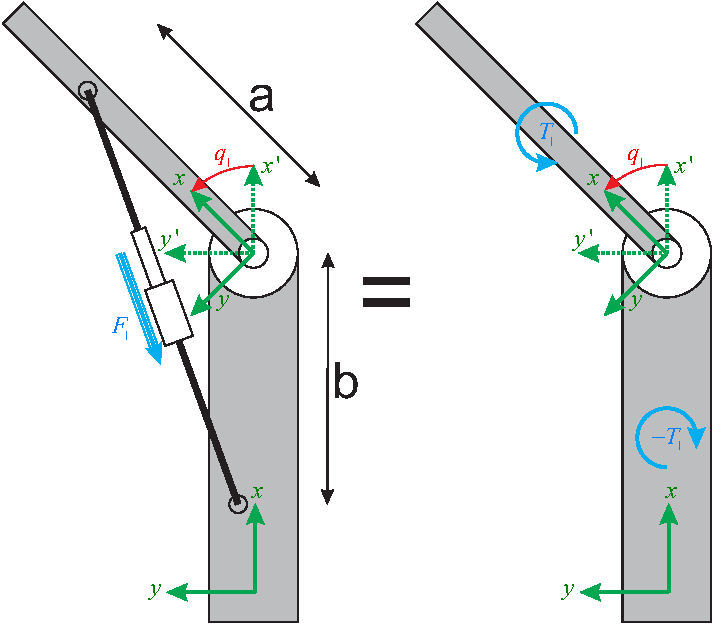
\includegraphics[width=0.6\textwidth]{../RobotArmExample/robotArm_cylinder.pdf}
	\caption{A cylinder in combination with a revolute joint has to be modeled as a torque actuator.}
	\label{fig:robotArmcylinder}
\end{figure}

The linear force $F_1$ with the two joint offsets $a,b$ can be transformed to a joint torque $T_1=f\left(q_1,a,b,F_1\right)$:
\begin{eqnarray}
\phi &=& \tan^{-1}\left(\frac{a\sin{q_1}}{b+a\cos{q_1}}\right) \\
T_1 &=& F_1 b\sin{\phi}
\end{eqnarray}


\section{Projected Newton-Euler Equations}
After the setup of the relative body kinematics (\secref{sec:kintree}) and the force elements (\secref{sec:forceel}) we can calculate the absolute kinematics and dynamics of the system by applying the projected Newton-Euler method:

\begin{lstlisting}
function [sys, body, ftel] = computePNE(body,ftel,q,dq,tau,I_a_grav)
 
% INPUT:
% * body:       kinematic tree
% * ftel:       force/torque elements
% * q:          generalized coordinates (symb) in desired order
% * Dq:         coresponding velocities
% * tau:        actuator force/torque array (symb)
% * I_a_grav:   gravity vector (R3)
%
% OUTPUT:
% * sys:        system struct containing dynamcis (all symbolic)
%   .MpNE:      mass matrix
%   .bpNE:      coriolis/centrifugal
%   .gpNE:      gravity terms
%   .SpNE:      actuator selection matrix
%   .fpNE:      =SpNE*T;
%   .param:     input parameters
%   .q:         generalized coordinates
%   .Dq:        generalized velocities
%   .tau        generalized actuator forces
%
% * body.kin:   body contains (among others) now also global kinematics as:
%   .A_IB:      rotation matrix from B to I (inertial/world frame)
%   .I_r_O:     vector inertial frame to body frame
%   .I_dr_O:    velocity of body frame in inertia frame
%   .I_r_CoG:   center of gravity position represented in inertia frame
%   .I_dr_CoG:  velcity ...
%   .I_J_CoG:   CoG jacobian
%   .I_Jr:      rotation jacobian
%   .I_Omega:   body rotational speed
%   ... and a lot more  

\end{lstlisting}


